Radio pulsars make up the majority of observations of neutron stars and will be
the focus of discussion in this thesis. In this section, we will provide some
population statistics for the normal radio pulsar population: we ignore the
millisecond population, but include the young pulsars. All data
in this section is taken from the ATNF pulsar catalogue \citet{ATNF} and it
should be stated that in each case the observed property is an average
over all observations made for each pulsar.

For each observable property of the population of neutron stars (such as the
frequency), we will present the data as a histogram choosing an appropriate
binning size in each instance. In order to make simple inferences about the
population, we also give the mean and standard-deviation and plot the
corresponding normal distribution.

In Fig.~\ref{fig: pop stats timing} we present the data for the three timing
properties measured directly from the pulsar timing models. For normal radio
pulsars the frequency, $f$, can always be accurately measured provided at least
one observation has been made.  Several precise observations of a pulsar must
be made in order to measure the higher order derivatives of the frequency. As a
result, the pulsar catalogue contains missing information and the number of
data points for $\dot{f}$ and $\ddot{f}$ is smaller than the total observed
number of pulsars: the exact numbers are given in the caption.
\begin{figure}[htb]
\centering
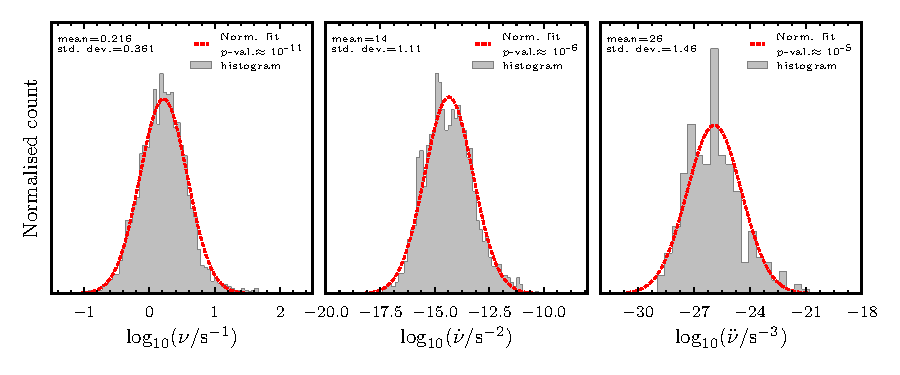
\includegraphics[]{timing_distribution}
\caption{The distribution in log-space of the frequency $f$ and the first two
frequency derivatives $\dot{f}$ and $\ddot{f}$ for normal radio pulsars in the
ATNF pulsar catalogue. Appropriate bin sizes were selected for each quantity.
The population sizes are 1942, 1686, 339 for $f$,
$\dot{f}$, $\ddot{f}$ respectively.}
\label{fig: pop stats timing}
\end{figure}

In Fig.~\ref{fig: pop stats others} we present some other interesting quantities
held in the ATNF catalogue. Firstly, in the left-hand panel we plot the characteristic
age as defined in Eqn.~\eqref{eqn: characteristic age}. Then, in the middle panel
we give a measure of the pulsars beam-width $W_{10}$. Specifically, $W_{10}$ is
the width of the integrated pulse profile (in seconds) at 10\% of the integrated
pulse profile maximum. In the right-hand panel we  plot $W_{10}f$, i.e. the
product of the beam-width and frequency for each pulsar. This gives information
about the effective duty-cycle: the ratio between the pulse duration and period.
Notably, the majority of pulsars have duty-cycles substantially less than a
$0.5$ indicating that the pulses are short compared to the period.
\begin{figure}[htb]
\centering
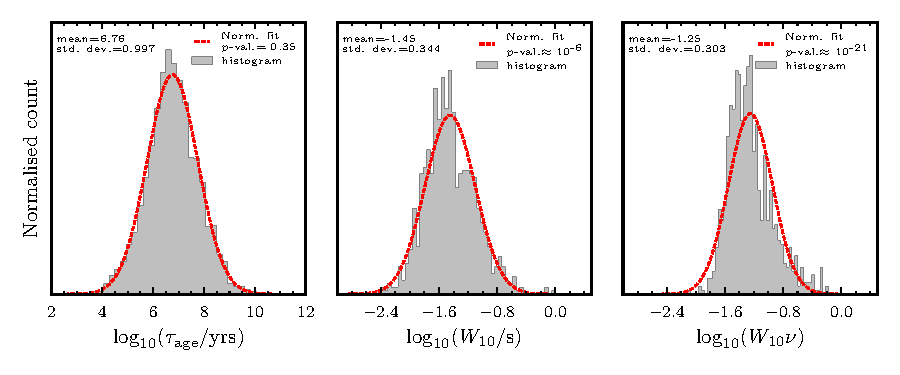
\includegraphics[]{W10_and_age_distribution}
\caption{The distribution in log-space of the characteristic age
$\tau_{\textrm{Age}}$, the $W_{10}$ measure of the beam-width, and the
effective duty-cycle $W_{10} f$ for normal radio pulsars in the
ATNF pulsar catalogue. Appropriate bin sizes were selected for each quantity.
The population sizes are 1942, 915, and 915 for
$\tau_{\textrm{Age}}$, $W_{10}$, and $W_{10}f$.}
\label{fig: pop stats others}
\end{figure}

